\documentclass[a4paper, 12pt]{article}
\usepackage{graphicx} % Required for inserting images
\usepackage{fullpage}
\usepackage{amsmath}
\usepackage{xcolor}
\usepackage{float}
\usepackage{geometry}
\usepackage{biblatex}
\geometry{margin=1in}
\usepackage{enumitem}
\usepackage{hyperref}
\usepackage{parskip}
\usepackage{pgfplots}
\pgfplotsset{compat=1.18}
\usepackage[normalem]{ulem}
\usepackage[version=4]{mhchem}

\title{Chemistry Honors Study Guide}
\author{Test 1 S2}
\date{Test date: February 14, 2025}

\begin{document}

\maketitle

\section{Limiting and Excess Reagents}

\subsection*{Definitions}

\begin{itemize}[leftmargin=*, nosep]
    \item \textbf{\textit{limiting (lim) reagent:}} The reactant that limits the amount of product yielded to a certain number.
    \item \textbf{\textit{excess (xs) reagent:}} The reactant left over after all of the limiting reagent is used.
    \item \textbf{\textit{theoretical yield:}} The theoretical amount of product produced found through calculations.
    \item \textbf{\textit{actual yield:}} The amount of product actually produced, likely affected by sources of error, found by doing the experiment. (Also \textit{experimental yield.})
    \item \textbf{\textit{percent yield:}} The percentage of the theoretical yield that is actually produced through experimentation.
\end{itemize}

\subsection*{Finding Limiting Reagent and Theoretical Yield}
A limiting reagent limits the amount of product that can be created in a chemical reaction (no matter how much of the other reactant you have, the limiting reagent controls the maximum reactant produced, known as theoretical yield). If you are making sandwiches and have 20 slices of bread but only 2 slices of cheese, it doesn't matter how much bread you have; you can only make 2 sandwiches, so the cheese is the limiting reagent, the bread is the excess reagent, and 2 is the theoretical yield.

Example:

$$2\text{HCl} + \text{Zn} \longrightarrow \text{ZnCl}_2 + \text{H}_2$$

If you react \textcolor{blue}{17 $g$ HCl} with \textcolor{blue}{17 $g$ Zn}, what is the limiting reagent and theoretical yield of ZnCl$_2$?

\textcolor{blue}{\textbf{Step 1:} Find how many grams of ZnCl$_2$} each reactant provides.

$$(17 \: g \: \text{HCl}) \times \left(\frac{1 \: mol \: \text{HCl}}{36.461 \: g \: \text{HCl}}\right) \times \left(\frac{1 \: mol \: \text{ZnCl}_2}{2 \: mol \: \text{HCl}}\right) \times \left(\frac{136.286 \: g \: \text{ZnCl}_2}{1 \: mol \: \text{ZnCl}_2}\right)$$

$$ \approx 31.77 \: g \: \text{ZnCl}_2$$

$$(17 \: g \: \text{Zn}) \times \left(\frac{1 \: mol \: \text{Zn}}{65.38 \: g \: \text{Zn}}\right) \times \left(\frac{1 \: mol \: \text{ZnCl}_2}{1 \: mol \: \text{Zn}}\right) \times \left(\frac{136.286 \: g \: \text{ZnCl}_2}{1 \: mol \: \text{ZnCl}_2}\right)$$

$$ \approx 35.44 \: g \: \text{ZnCl}_2$$

\textcolor{blue}{\textbf{Step 2:} Find the limiting reagent} by taking the element that produces the smallest amount of the product (the theoretical yield). The excess reagent is the other reactant.

\fbox{
\begin{minipage}{0.4\textwidth} 
limiting reagent: HCl \\ 
excess reagent: Zn \\ 
theoretical yield: 31.77 g ZnCl$_2$ 
\end{minipage}}

\subsection*{Finding Percent Yield}
To find the percent yield, use this formula:

$$\frac{\text{actual yield}}{\text{theoretical yield}} \times 100\%$$

\subsection*{Finding Amount of Excess Reagent}
To find the amount of excess reagent left over after a reaction has occurred, work backwards from the theoretical yield.

Example:

$$\text{Al} + \text{MgCl}_2 \longrightarrow \text{AlCl}_3 + \text{Mg}$$

If you react \textcolor{blue}{10 $g$ Al} with \textcolor{blue}{10 $g$ MgCl$_2$}, how many grams of excess reagent are there?

\textcolor{blue}{\textbf{Step 1:} Always check if the equation is balanced}, and if not, balance it.

$$\text{2Al} + \text{3MgCl}_2 \longrightarrow \text{2AlCl}_3 + \text{3Mg}$$

\textcolor{blue}{\textbf{Step 2:} Find the theoretical yield} by applying the steps shown in the prior example.

$$(10 \: g \: \text{Al}) \times \left(\frac{1 \: mol \: \text{Al}}{26.982 \: g \: \text{Al}}\right) \times \left(\frac{2 \: mol \: \text{AlCl}_3}{2 \: mol \: \text{Al}}\right) \times \left(\frac{133.341 \: g \: \text{AlCl}_3}{1 \: mol \: \text{AlCl}_3}\right)$$

$$ \approx 49.42 \: g \: \text{AlCl}_3$$

$$(10 \: g \: \text{MgCl}_2) \times \left(\frac{1 \: mol \: \text{MgCl}_2}{95.211 \: g \: \text{MgCl}_2}\right) \times \left(\frac{2 \: mol \: \text{AlCl}_3}{3 \: mol \: \text{MgCl}_2}\right) \times \left(\frac{133.341 \: g \: \text{AlCl}_3}{1 \: mol \: \text{AlCl}_3}\right)$$

$$ \approx 9.34 \: g \: \text{AlCl}_3 \longleftarrow \text{\textcolor{red}{theoretical yield, lim. reagent is MgCl$_2$}}$$

\textcolor{blue}{\textbf{Step 3:} Work backwards from the theoretical yield} and find how many grams of excess reagent (Al) is needed to produce approximately 9.3 grams of AlCl$_3$.

$$(9.3 \: g \: \text{AlCl}_3) \times \left(\frac{1 \: mol \: \text{AlCl}_3}{133.341 \: g \: \text{AlCl}_3}\right) \times \left(\frac{2 \: mol \: \text{Al}}{2 \: mol \: \text{AlCl}_3}\right) \times \left(\frac{26.982 \: g \: \text{Al}}{1 \: mol \: \text{Al}}\right)$$

$$\approx 1.88 \: g \: \text{Al}$$

\textcolor{blue}{\textbf{Step 4:} Subtract this number} from the amount of aluminum used in the reaction to get $10 - 1.88 = \boxed{8.12 \: g}$ of excess reagent.

\textcolor{blue}{\textbf{Step 5:} Check if the answer is reasonable.} There was a large difference between the product yielded by the magnesium chloride and the aluminum, so it makes sense that there is a significant amount of aluminum left over.

\section{Ionic Reactions}

\subsection*{Types of Reactions} \label{types of reactions}

\paragraph{Combination reaction}
Two or more reactants combine to create one product
$$ A + B \longrightarrow AB$$

\paragraph{Decomposition reaction}
Reactant decomposes into two or more products
$$ AB \longrightarrow A + B$$ 

\paragraph{Double displacement reaction}
Two ionic compounds switch anions
$$ AB + CD \longrightarrow AD + CB$$ 

\paragraph{Single displacement reaction}
The anion switches from one reactant to the other (note: when predicting products, diatomic elements that stand alone should have 2 as a subscript)
$$ A + BC \longrightarrow AC + B$$ 

\paragraph{Combustion reaction}
Substance reacts with oxygen, creating energy (heat)
$$ \text{C}_x\text{H}_y + \text{O}_2 \longrightarrow \text{H}_2\text{O} + \text{CO}_2$$

\paragraph{Neutralization reaction}
An acid reacts with a base to form water and an ionic compound

$$\text{H}A + B\text{OH} \longrightarrow \text{H$_2$O +} BA $$

\subsection*{Ionic Equations}

\textbf{Balanced chemical eqn. (B.C.E.) or molecular equation}

$$2\text{AgNO}_{3(aq)} + \text{CuCl}_{2(aq)} \longrightarrow 2\text{AgCl}_{(s)} + \text{Cu(NO$_3$)}_{2(aq)}$$

\textbf{(Overall) ionic eqn. (I.E.):} break apart aq. compounds (bring subscript to the front)

$$2\text{Ag}^+ + 2{\text{NO}_3}^- + \text{Cu}^{2+} + 2\text{Cl}^- \longrightarrow 2\text{AgCl} + \text{Cu}^{2+} + {2\text{NO}_3}^-$$

(do not need subscripts)

Compounds that can be cancelled out (\textbf{spectator ions}) are not involved in the reaction. ($2\text{NO}_3^-$ and $\text{Cu}^{2+}$)

\textbf{Net ionic eqn. (N.I.E.):} get rid of compounds that cancel out (should be charge-balanced)

$$2\text{Ag}^+ + 2\text{Cl}^- \longrightarrow 2\text{AgCl}$$

This is the actual reaction that occurs.

\textcolor{red}{No net ionic equation, all spectator ions, all aqueous = NO REACTION}

\textbf{Precipitation rxn w/ ppt (precipitate, $(s)$)}

$$(aq) + (aq) \longrightarrow (s) + (aq)$$

\subsection*{Solubility Rules} \label{solubility rules}
These rules are provided on tests and quizzes and do not need to be memorized. Soluble = aqueous, insoluble = solid.

\begin{enumerate}[leftmargin=*, nosep]
    \item Alkali metals (group 1) are always soluble.
    \item Ammonium, (NH$_4$$^+$) is always soluble.
    \item Nitrates (NO$_3$$^-$), chlorates (Cl$_3$$^-$), and perchlorates (ClO$_4$$^-$)
    \item Most hydroxides (OH$^-$) are insoluble except those paired with an alkali metal or barium.
    \item Most chlorides (Cl$^-$), bromides (Br$^-$), and iodides chlorides (I$^-$) are soluble except when they are paired with silver (Ag$^+$), lead (Pb$^{2+}$), and mercury (Hg$^{2+}$).
    \item Carbonates (CO$_2$$^{3-}$), phosphates (PO$_4$$^{3-}$), and sulfides (S$^{2-}$) are insoluble except when paired with ammonium (NH$_4$$^+$) and alkali metals.
    \item Most sulfates (SO$_4$$^{2-}$) are soluble except barium sulfate (BaSO$_4$), lead sulfate (PbSO$_4$), and mercury sulfate (HgSO$_4$).
\end{enumerate}

\section{Solutions}

\subsection*{Definitions}

\begin{itemize}[leftmargin=*, nosep]
    \item \textbf{\textit{solution:}} A homogeneous mixture in the liquid phase.
    \item \textbf{\textit{solvent:}} The larger part of the solution in the liquid phase.
    \item \textbf{\textit{solute:}} The smaller part of the solution that is dissolved in the solvent. Can be solid, liquid, or gas.
    \item \textbf{\textit{percent by mass:}} The percentage of the solution that is the solvent.
    \item \textbf{\textit{molarity:}} How many moles of dissolved solute is present per liter of solution.
    \item \textbf{\textit{dilution:}} To make a solution less concentrated.
\end{itemize}

\subsection*{Calculating Concentration}

$$ \text{\textbf{Percent by mass}} = \frac{\text{mass of solute}}{\text{mass of solution}} \times 100\%$$

$$ \text{\textbf{Molarity} or $\frac{mol}{L}$ or $M$} = \frac{\text{moles of solute}}{\text{liters of solution}} \times 100\%$$

(units of molarity are $\frac{mol}{L}$ or $M$)

Example: If you dissolve \textcolor{blue}{6.3 $g$ NaCl} in \textcolor{blue}{92 $g$ H$_2$O}, the resulting solution has a volume of 90 $ml$. What is the percent by mass of the solute and the molarity?

\textcolor{blue}{\textbf{Step 1:} Find the percent by mass} using the formula above.

$$\frac{6.3 \: g \: \text{NaCl}}{98.3 \: g \: \text{H$_2$O}} \times 100\% = 6.41 \%$$

\textcolor{blue}{\textbf{Step 2:} Find the number of moles} of solute with the molar mass of NaCl.

$$(6.3 \: g) \times \left(\frac{1 \: mol}{58.44 \: g}\right) = 0.11 \: mol \: \text{NaCl}$$

\textcolor{blue}{\textbf{Step 3:} Calculate molarity} using the formula above.

$$\frac{0.11 \: mol \: \text{NaCl}}{0.09 \: L} = 1.22 \: M$$

\fbox{
\begin{minipage}{0.3\textwidth} 
percent by mass: 6.41\% \\
molarity: 1.22 $M$
\end{minipage}}

\subsection*{Dilution}

$$C_1V_1 = C_2V_2$$

where:

$C_1$ is the concentration of the stock solution (more concentrated);\\
$V_1$ is its volume;\\
$C_2$ is the concentration of the diluted solution;\\
$V_2$ is its volume.

Example: How many ml of \textcolor{blue}{12 $M$ HCl} do you need to make \textcolor{blue}{250 ml} of \textcolor{blue}{0.5 $M$ HCl}?

$$C_1V_1 = C_2V_2$$
$$(12\: M)V_1 = (0.5 \: M)(250 \: ml)$$
$$ = \boxed{10.4 \: ml}$$

\subsection*{Solution Stoichiometry}
How many liters of \textcolor{blue}{0.5 $M$ H$_2$SO$_4$} are needed to fully react with \textcolor{blue}{0.25 $L$} of \textcolor{blue}{0.75 $M$ NaOH?}

\textcolor{blue}{\textbf{Step 1:} Set up the balanced chemical equation} with coefficients and subscripts, determining subscripts using solubility rules (page \pageref{solubility rules}) and predicting products using types of reactions (page \pageref{types of reactions}).

$$\text{H}_2\text{SO}_{4(aq)} + 2\text{NaOH}_{(aq)} \longrightarrow 2\text{H$_2$O}_{(l)} + \text{Na$_2$SO$_4$}_{(aq)}$$

\textcolor{blue}{\textbf{Step 2:} Using molarity as a conversion factor, convert to moles}, then perform the usual calculation.

$$(0.25 \: L \: \text{NaOH}) \times \left(\frac{0.75 \: mol \: \text{NaOH}}{1 \: L}\right) \times \left(\frac{1 \: mol \: \text{H$_2$SO$_4$}}{2 \: mol \: \text{NaOH}}\right) \times \left(\frac{1 \: L \: \text{H$_2$SO$_4$}}{0.5 \: mol \: \text{H$_2$SO$_4$}}\right)$$

$$= \boxed{0.1875 \: L \: \text{H$_2$SO$_4$}}$$

\section{Acids and Bases}

\subsection*{Definitions}
\begin{itemize}[leftmargin=*, nosep]
    \item \textbf{\textit{Arrhenius acid:}} Releases H$^+$ into the solution (starts with H).\footnote{The exception to this is water; it is an \textbf{ampholyte} (\textbf{amphoteric}, able to act both as an acid and a base)}.
    \item \textbf{\textit{Arrhenius base:}} Releases OH$^-$ into the solution (ends with OH).
    \item \textbf{\textit{Bronsted-Lowry acid:}} A proton (H$^+$) donor.
    \item \textbf{\textit{Bronsted-Lowry base:}} A proton acceptor. Does not necessarily have to end with OH.\footnote{A square is always a rectangle, but a rectangle is not always a square. Similarly, an Arrhenius base is always a Bronsted-Lowry base, but a Bronsted-Lowry base is not always an Arrhenius base.}
    \item \textbf{\textit{titration:}} A laboratory technique, adding a substance with known concentration to a second substance with unknown concentration to determine the concentration or identity of the second.
    \item \textbf{\textit{titrant:}} The substance in a titration with known concentration.
    \item \textbf{\textit{analyte:}} The substance in a titration with unknown concentration.
    \item \textbf{\textit{monoprotic acid:}} An acid that begins with 1 hydrogen atom.
    \item \textbf{\textit{diprotic acid:}} An acid that begins with 2 hydrogen atoms.
    \item \textbf{\textit{monobase:}} A base that ends with 1 hydroxide molecule.
    \item \textbf{\textit{dibase:}} A base that ends with 2 hydroxide molecules.
\end{itemize}

\subsection*{pH and pOH}
pH and pOH are negative log scales, so as they increase by 1 integer, the concentration of H$^+$ or OH$^-$ decreases by tenfold. For example, a substance with pH 3 has 10 times the H$^+$ concentration as a substance with pH 4.

These are the three formulas:

\textbf{Formula for pH:}
\begin{equation}\label{pH}
    \text{pH} = -\log[\text{H$^+$}]
\end{equation}

\textbf{Formula for pOH:}
\begin{equation}\label{pOH}
\text{pOH} = -\log[\text{OH$^-$}]
\end{equation}

\textbf{Relationship between pH and pOH:}
\begin{equation}\label{pHandpOH}
    \text{pH} + \text{pOH} = 14
\end{equation}

And these are the formulas that are derived from the above:

\textbf{Derived from} \ref{pH}:
$$ \text{[H$^+$] = 10$^{-\text{pH}}$}$$

\textbf{Derived from} \ref{pOH}:
$$ \text{[OH$^-$] = 10$^{-\text{pOH}}$}$$

\textbf{Derived from} \ref{pHandpOH}:
$$14 - \text{pOH} = \text{pH}$$
$$14 - \text{pH} = \text{pOH} $$

The pH scale ranges from 0 to 14, with 0 being the most acidic, 14 being the most basic, and 7 being neutral (water).

The pOH scale also ranges from 0 to 14 but works in the opposite direction, with 0 being the most basic, 14 being the most acidic, and 7 being neutral.

\subsection*{Strong/Weak Acids and Bases}
Strong acids/bases dissociate fully (use $\longrightarrow$ for dissociation reaction) and weak acids/bases do not dissociate fully (use $\rightleftharpoons$ for dissociation reaction).

The strong acids will be given on the test. Strong bases are \textbf{groups 1+2 OH$^-$.}

\textbf{When an acid or base is strong, the molarity of H$^+$ or OH$^-$ is equal to the molarity of the original compound.} For example:

$$ \text{HCl} \longrightarrow \text{H$^+$ + Cl$^-$}$$

This is a strong acid, so [H$^+$] = [HCl]. For the dissociation of a weak acid/base, the concentrations are not equal.

\subsection*{Dissociation reactions}

\textbf{Diprotic dissociation:}
$$\text{First dissociation: H$_2$CO$_3$}\rightleftharpoons \text{H$^+$} + \text{HCO$_4$$^-$}$$
$$\text{Second dissociation: HCO$_3$$^-$} \rightleftharpoons \text{H$^+$} + \text{CO$_3$$^{2-}$}$$

$\rightleftharpoons$ denotes a reversible reaction and should be used when a weak acid/base is present.

\textbf{Overall dissociation:}
$$\text{H$_2$CO$_3$}\rightleftharpoons \text{2H$^+$} + \text{CO$_3$$^{2-}$}$$

\subsection*{Conjugate Acids and Bases}

$$\text{NH}_3 + \text{HCl} \longrightarrow \text{NH$_4$$^+$} + \text{Cl}^-$$

\textbf{acid}, HCl, \textit{donates a proton} (H$^+$) to become the \textbf{conjugate base}, Cl$^-$

\textbf{base}, NH$_3$, \textit{accepts a proton} to become the \textbf{conjugate acid} (NH$_4$$^+$)

\subsection*{Naming Acids}
Acids are named by their anions\footnote{Keep prefixes (e. g. hypo-, per-)} because they all begin with H.

\begin{table}[H]
    \centering
    \begin{tabular}{c|c|c}
        \textbf{Anion suffix} & \textbf{Acid suffix} & \textbf{Mnemonic device} \\\hline
        -ide & hydro- -ic & My r\underline{ide} has \underline{hydr}aul\underline{ic}s\\
        -ate & -ic & I \underline{ate} some \underline{ic}ky acid \\
        -ite & -ous & Dynam\underline{ite} is danger\underline{ous}\\ 
    \end{tabular}
    \label{tab:namingacids}
\end{table}

\subsection*{Acid-Base Titrations}
Acid-base titrations are the most common type of titration and are done by titrating an acid with a strong base or a base with a strong acid.

\begin{center}
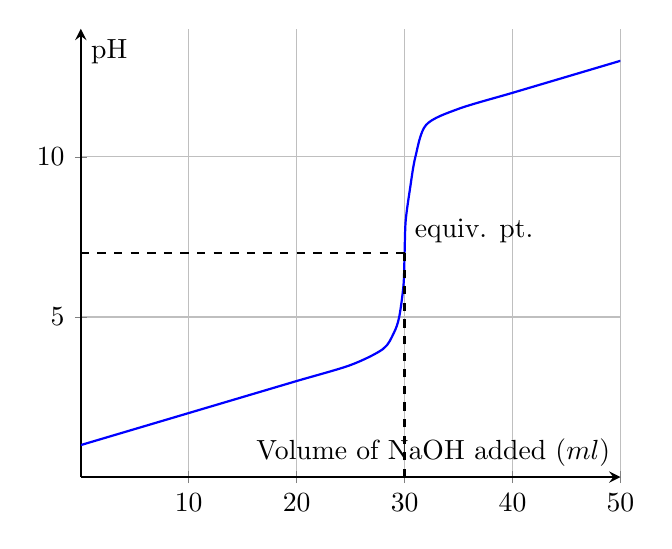
\begin{tikzpicture}
    \begin{axis}[
        xlabel={Volume of NaOH added ($ml$)},
        ylabel={pH},
        xmin=0, xmax=50,
        ymin=0, ymax=14,
        samples=100,
        thick,
        domain=0:50,
        grid=major,
        axis lines=middle
    ]
    % Titration curve for strong acid-strong base
    \addplot[blue, smooth] 
    coordinates {
        (0,1) (5,1.5) (10,2) (15,2.5) (20,3) (25,3.5) (28,4) 
        (29,4.5) (29.5,5) (29.9,6) (30,7) (30.1,8) (30.5,9) (31,10)
        (32,11) (35,11.5) (40,12) (45,12.5) (50,13)
    };
    
    % Mark equivalence point
    \draw[dashed] (0,7) -- (30,7) node[above right] {equiv. pt.};
    \draw[dashed] (30, 0) -- (30, 7);
    
    \end{axis}
\end{tikzpicture}
\end{center}

When performing a titration, try to aim for a light pink color. The \textbf{equivalence point} of a monobase/monoprotic acid is at pH = 7. For dibases/diprotic acids, there are 2 equivalence points, and the pH at these points varies.

\subsubsection*{Titration Stoichiometry}
You use \textcolor{blue}{0.5 $M$ NaOH} to titrate a monoprotic acid. It takes \textcolor{blue}{15 $ml$ NaOH} to reach the equivalence point, and you started with \textcolor{blue}{25 $ml$} of acid. What is the acid concentration?

\textcolor{blue}{\textbf{Step 1:} Write and balance} the chemical formula.

$$\text{NaOH} + \text{HCl} \longrightarrow \text{H$_2$O} + \text{NaCl}$$

\textcolor{blue}{\textbf{Step 2:} Calculate the number of moles} of acid that you have.

$$(0.015 \: L \: \text{NaOH}) \times \left(\frac{0.5 \: mol \: \text{NaOH}}{1 \: L \: \text{NaOH}}\right) \times \left(\frac{1 \: mol \: \text{HCl}}{1 \: mol \: \text{NaOH}}\right) $$
$$=0.0075 \: mol \: \text{HCl}$$

\textcolor{blue}{\textbf{Step 3:} Put this number over the number of liters of acid you started with} to find the concentration (molarity).

$$\frac{0.0075 \: mol \: \text{HCl}}{0.025 \: L} = \boxed{0.3 \: M \: \text{HCl}}$$

\end{document}
